\documentclass{beamer}

%style
\mode<presentation>
\usetheme{Boadilla}

%Packages
\usepackage[utf8]{inputenc}
\usepackage[ngerman]{babel}
\usepackage{graphicx}
\usepackage{booktabs}
\usepackage{mathtools}
\usepackage{amsmath}
\usepackage{listings}
\usepackage[utf8]{inputenc}
\usepackage[ngerman]{babel}
\usepackage[T1]{fontenc}
\usepackage{lmodern}
\usepackage{tabto}
\usepackage{listings}
\usepackage{framed} 
\usepackage{xcolor} 
\colorlet{shadecolor}{gray!25}
%bibtex
\usepackage[backend=biber, style=authoryear]{biblatex}
\addbibresource{referenzen.bib}

%Einstellungen der Präsentation
\title[Netzwerk und Systemsicherheit]{Log4J zu Log4Shell}
\subtitle{Netzwerk und Systemsicherheit}
\author{Moritz Rupp}
\institute[MR]{Hochschule Albstadt-Sigmaringen}
\setbeamertemplate{navigation symbols}{}%remove navigation symbols
\date{WS 21/22}

%Beginn der Präsentation
\begin{document}

%Titelseite
\begin{frame}
\titlepage
\end{frame}
%Inhaltsverzeichnis
\begin{frame}
\frametitle{Inhalt}
\tableofcontents    
\end{frame}
\section{Was ist Log4J und Log4Shell?}
\begin{frame}{Was ist Log4J?}
\begin{itemize}
 \item Java Framework zum Loggen von Anwendungsmeldungen\\
 - Open Source
 \item Entwickelt ab 1996 bei IBM
 \item Seit anfang 2000 der Standart für Logging\\
 \item Verwendung auf allen relevanten Plattformen\\
 $\Rightarrow$ Windows, Linux, MacOs\\
 $\Rightarrow$ Läuft auf über 3 Milliarden Geräten
 \item Adaption der Log4J Konzepte von vielen Programmiersprachen\\
 - Log4C, Log4cplus, Log4js, Logging in Python 
 \item Betreuung durch das Apache Logging Projekt
\end{itemize}
\end{frame}
\begin{frame}{Was ist Log4Shell?}
\begin{itemize}
\item Zero-Day Sicherheitslücke in der Log4J Biblothek
\item Erster Report Ende November 2021 durch Mitarbeiter bei Alibaba 
\item Veröffentlichung am 10. Dezember 2021 unter CVE-2021-44228
\item Ermöglicht Arbitary Code Execution\\
$\Rightarrow$ Remote Code Exection, Reverse Shell etc.
\item BSI stuft Log4shell mit Bedrohungslage 4/Rot ein

\end{itemize}
\begin{center}
 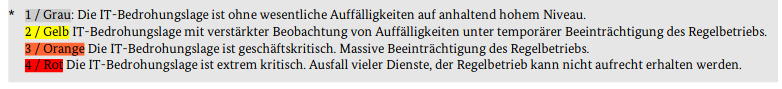
\includegraphics[scale=0.35]{bsilog4j.png}
\end{center}


 
\end{frame}
\section{Trivia}
\begin{frame}{Trivia}
 \begin{itemize}
  \item Über 3 Milliarden Geräte potenziell Betroffen
  \item Gilt als größte Sicherheitslücke seit Shellshock
  \item Nach wie vor im Umlauf
  \item Mehrere Großte It Infrastrukuren betroffen
  
  
 \end{itemize}

\end{frame}


\begin{frame}{Funktionsweiße}
 
\end{frame}







\end{document}

